\documentclass{templateNote}
\usepackage{tcolorbox}
\usepackage{pgfplots}
\usepackage{pgf-pie}
\usepackage{tabularx}

\newcolumntype{L}{>{\centering\arraybackslash}X}

\begin{document}

\imagenlogo{img/LogoElNube.png}
\universidad{Universidad del Bío-Bío}
\titulo{Practico 2} % Titulo
\asignatura{Estadistica y Probabilidades} % Asignatura
\autor{
    \indent
    Marcelo \textsc{Paz}
}   
\portada
\margenes % Crear márgenes


% \section{Teoria}
% \indent
% aqui el texto

% \newpage

\section{Ejercicios}
Clasifique las siguientes variables. Indique si son cualitativas o cuantitativas. Si son cuantitativas, indique si corresponde a una variable discreta o continua.
\begin{samepage}
    \subsection{1 Estudio de Anorexia}
    \indent
    Según la Asociación de lucha contra la Bulimia y la Anorexia, las pautas culturales
    han determinado que la delgadez sea sinónimo de éxito social. Muchos jóvenes luchan para
    conseguir el “físico ideal” motivados por modelos, artistas o por la publicidad comercial.
    Durante el mes de marzo del año 2006, en el colegio “Alcántara” de la ciudad de Talca,
    después de las vacaciones de verano, se observó con precaución a 27 alumnos con síntomas
    de anorexia, registrándose los siguientes signos visibles:

    \begin{table}[H]
        \begin{center}
            \begin{tabular}{| c | c | c |}
                \hline Dieta Severa & Miedo a Engordar & Hiperactividad \\
                Uso de Ropa Holgada & Dieta Severa & Uso de Laxantes \\
                Miedo a Engordar & Dieta Severa & Uso de Ropa Holgada \\
                Dieta Severa & Uso de Ropa Holgada & Dieta Severa \\
                Dieta Severa & Dieta Severa & Uso de Ropa Holgada \\
                Hiperactividad & Uso de Laxantes & Miedo a Engordar \\
                Uso de Laxantes & Dieta Severa & Uso de Ropa Holgada \\
                Uso de Laxantes & Hiperactividad & Uso de Laxantes \\
                Uso de Ropa Holgada & Hiperactividad & Dieta Severa \\ \hline
            \end{tabular}
            \caption{Estudio de Anorexia}
        \end{center}
    \end{table}

    
    \subsubsection{a}
    \indent
    Resuma la información anterior en una tabla de distribución de frecuencias que además contenga la frecuencia relativa porcentual.
    
    \begin{table}[H]
        \begin{center}
            \begin{tabular}{| c | c | c |}
                \hline
                Signos Visibles & Frecuencia $f_i$ & Frecuencia Relativa porcentual $fr_i$ \\
                \hline
                Dieta Severa & 9 & 33\% \\
                Uso de Ropa Holgada & 6 & 22\% \\
                Miedo a Engordar & 3 & 11\% \\
                Hiperactividad & 4 & 15\% \\
                Uso de Laxantes & 5 & 19\% \\
                \hline
                Total & 27 & 100\% \\
                \hline
            \end{tabular}
            \caption{Distribución de frecuencias}
        \end{center}
    \end{table}
\end{samepage}
\newpage
\subsubsection{b}
\indent
Grafique de manera adecuada la información de la tabla.

\begin{figure}[H]
    \begin{center}
        \caption{Signos Visibles}
        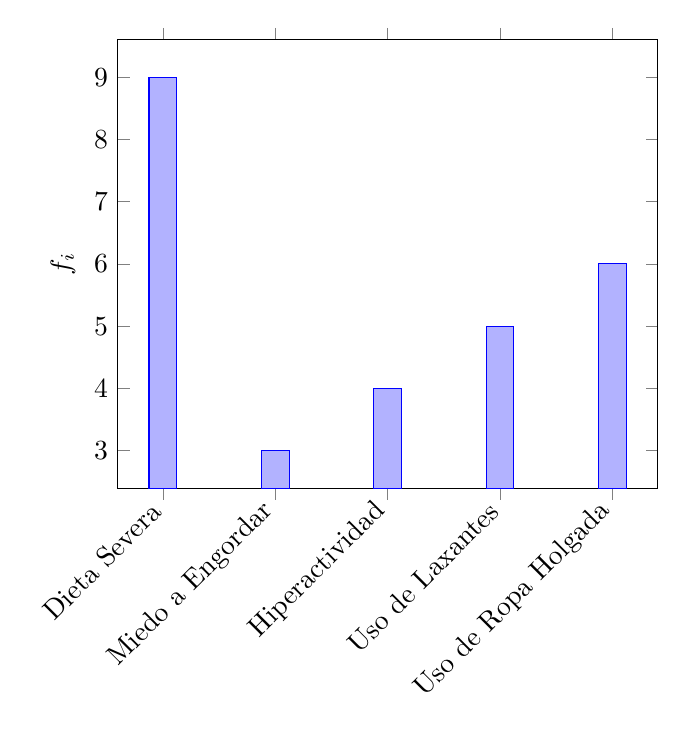
\begin{tikzpicture}
            \begin{axis}[xtick=data, % Para que cada barra tenga una etiqueta
                        xticklabels={Dieta Severa, Miedo a Engordar, Hiperactividad, Uso de Laxantes, Uso de Ropa Holgada},
                        xticklabel style={rotate=45,anchor=east},
                        ytick distance=1, % Para que la distancia entre cada marca del eje y sea de 1
                        ylabel={$f_i$},
                        ybar]
                \addplot coordinates {(1,9) (2,3) (3,4) (4,5) (5,6)};
            \end{axis}
        \end{tikzpicture}
    \end{center}
\end{figure}

\begin{figure}[H]
    \begin{center}
        \caption{Signos Visibles}
        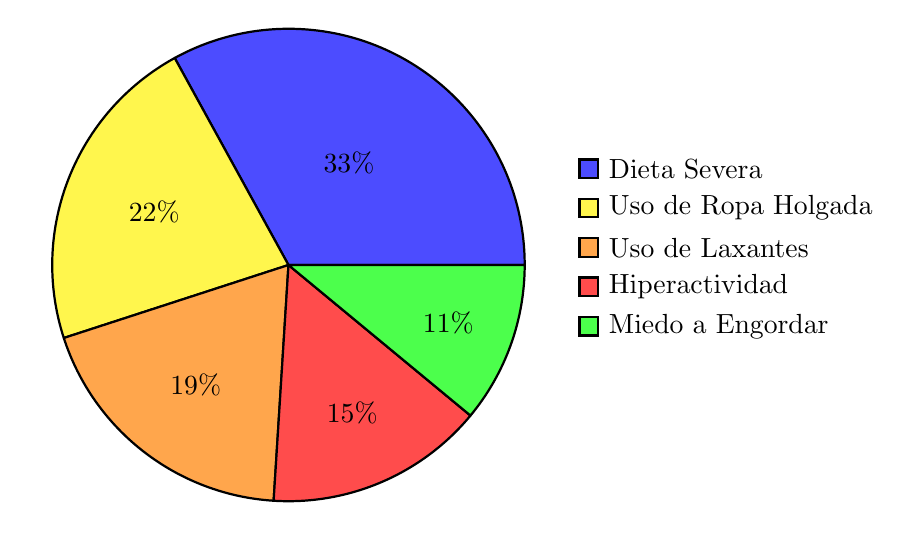
\begin{tikzpicture}
            \pie[text=legend, color={blue!70, yellow!70, orange!70, red!70, green!70}]{33/Dieta Severa, 22/Uso de Ropa Holgada, 19/Uso de Laxantes, 15/Hiperactividad, 11/Miedo a Engordar}
        \end{tikzpicture}
    \end{center}
\end{figure}


\subsubsection{c}
\indent
¿Qué medida de centralización es adecuada para estos datos? Comente e interprete adecuadamente.

\textbf{R:} La única medida de tendencia central que se puede obtener en una variable cualitativa
es la moda.

\newpage
\begin{samepage}
    
    \subsection{2 Asignaturas reprobadas}
    \indent
    Las siguientes observaciones corresponden al número de asignaturas reprobadas por un
    grupo de alumnos de la carrera de Ingeniería de la Universidad (no se ha considerado la
    especialidad)
    \begin{table}[H]
        \begin{center}
            \begin{tabular}{| c | c | c | c | c | c | c | c | c | c | c | c | c | c | c | c | c | c |}
                \hline
                5 & 0 & 2 & 0 & 0 & 0 & 3 & 0 & 0 & 0 & 1 & 6 & 4 & 3 & 3 & 1 & 4 & 0 \\
                1 & 7 & 5 & 0 & 0 & 4 & 3 & 6 & 2 & 0 & 3 & 1 & 2 & 2 & 0 & 0 & 0 & 1 \\
                0 & 3 & 1 & 1 & 0 & 1 & 0 & 1 & 0 & 1 & 0 & 2 & 0 & 0 & 4 & 4 & 2 & 2 \\
                2 & 2 & 0 & 0 & 0 & 1 & 2 & 2 & 0 & 2 & 3 & 4 & 5 & 2 & 2 & 2 & 2 & 1 \\
                1 & 2 & 1 & 1 & 1 & 1 & 3 & 2 & 2 & 2 & 2 & 3 & 3 & 3 & 4 & 5 & 6 & 0 \\
                \hline
            \end{tabular}
            \caption{Asignaturas reprobadas}
        \end{center}
    \end{table}
    \subsubsection{a}
    \indent
    Reconozca y clasifique la variable de interés.
    \textbf{R:} La variable de interés es el número de asignaturas reprobadas por un grupo de alumnos de la carrera de Ingeniería de la Universidad, la cual tiene una clasificación cuantitativa discreta.
    
    \subsubsection{b}
    \indent
    Agrupe los datos en una tabla de distribución de frecuencias.
    
    \begin{table}[H]
        \begin{center}
            \begin{tabularx}{\textwidth}{|L|L|L|L|}
                \hline
                Número de asignaturas reprobadas $c_i$ & Frecuencia Absoluta $f_i$ & Frecuencia Acumulada $F_i$ & Frecuencia Relativa porcentual $fr_i$ \\
                \hline
                0 & 26 & 26 & 28,8\% \\
                1 & 17 & 43 & 18,8\% \\
                2 & 21 & 64 & 23,3\% \\
                3 & 11 & 75 & 12,2\% \\
                4 & 7 & 82 & 7,7\% \\
                5 & 4 & 86 & 4,4\% \\
                6 & 3 & 89 & 3,3\% \\
                7 & 1 & 90 & 1,1\% \\
                \hline
                Total & 90 & & 100\% \\
                \hline
            \end{tabularx}
            \caption{Distribución de frecuencias}
        \end{center}
    \end{table}
    
\end{samepage}
\newpage
\subsubsection{c}
\indent
Grafique la información tabulada.

\begin{figure}[H]
    \begin{center}
        \caption{Asignaturas reprobadas}
        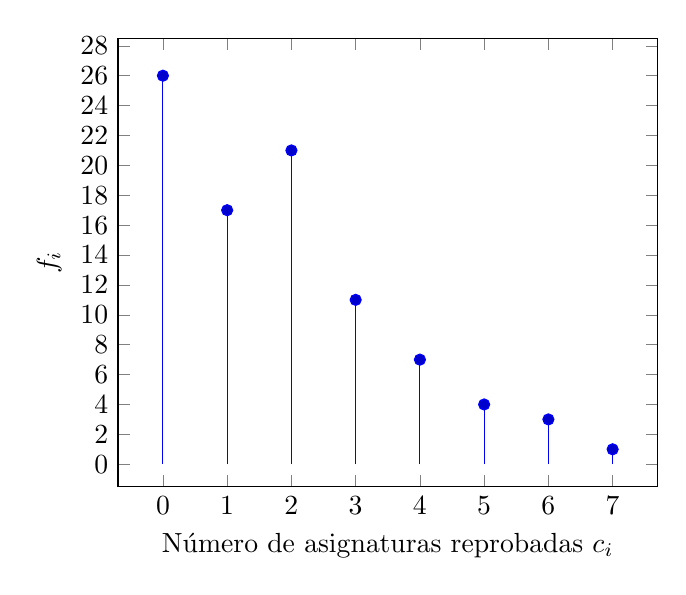
\begin{tikzpicture}
            \begin{axis}[
                xtick distance=1,
                ytick distance=2,
                xlabel={Número de asignaturas reprobadas $c_i$},
                ylabel={$f_i$}
            ]
            \addplot+[ycomb] plot coordinates
            {(0,26) (1,17) (2,21) (3,11) (4,7) (5,4) (6,3) (7,1)};
            \end{axis}
        \end{tikzpicture}
    \end{center}
\end{figure}

\subsubsection{d}
\indent
Calcule a partir de la tabla media, moda y mediana.
\[
    \bar{X} = \sum_{i=1}^{k} \frac{c_i \times f_i}{n} = \frac{0 \times 26 + 1 \times 17 + 2 \times 21 + 3 \times 11 + 4 \times 7 + 5 \times 4 + 6 \times 3 + 7 \times 1}{90} = 1,8
\]

\[
    M_o = 0
\]

\[
    \frac{n}{2} = \frac{90}{2} = 45 \Rightarrow M_e = 2
\]


\end{document}